\section{Veröffentlichung von Inhalten}
\frame{
 \frametitle{Veröffentlichung von Inhalten}
 Nicht jede*r Plonenutzer*in darf veröffentlichen 
 Für diese User übernimmt Referat ÖA die externe Veröffentlichung
 \subsection{Workflow}
 \begin{itemize}
 \item Referat xy erstellt Termin/Beitrag nach den inhaltlichen Regeln des StuRa
 \item Der Termin/Beitrag wird zur Veröffentlichung eingereicht
 \item Referat ÖA prüft Termin/Beitrag und nimmt bei Bedarf kleinere redaktionelle Änderungen und Korrekturen vor.
(Bei groben Fehlern wird der Termin/Beitrag zurückgewiesen)
\item Referat ÖA überprüft Kategorisierung und Relevanz für zusätzliche Veröffentlichung auf den Social       Media Sites.
\item Referat ÖA veröffentlicht den Termin/Beitrag extern.
\item Referat xy ist für die Verfolgung seiner Termine/Beiträge eigenverantwortlich.
\end{itemize}
}
\frame{
	\frametitle{Veröffentlichung von Inhalten}
    \begin{figure}[!h]
        \centering
        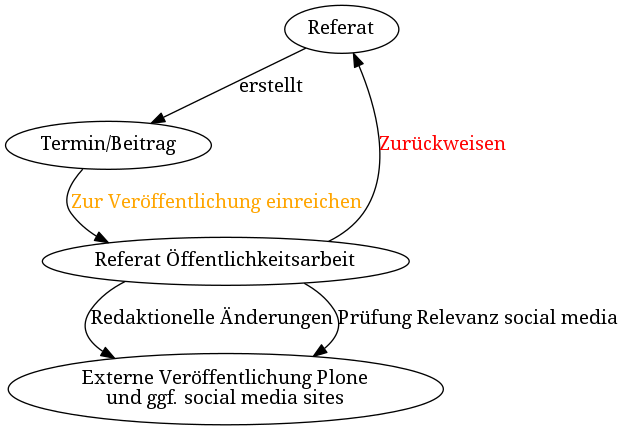
\includegraphics[height=0.8\textheight]{../res/veroeffentlichung.png}
    \end{figure}
}


\subsection{Inhalt}
\frame{
 \frametitle{Inhalt}
 Was muss vermieden werden:
 \begin{itemize}
 \item Generisches Maskulinum
 \item Fehler jeder Art
 \item Falsche Daten oder Ortsbezeichnungen
 \item Bilder ohne notwendige Rechte
 \item Falsche Verwendung von Logos
 \item Falsche oder fehlende Kategorisierung
 \item Satzzeichen, die in Rudeln auftreten 
 \end{itemize}
}
